\section{Desenvolvimento}
\label{desenvolvimento}

Essa seção, as vezes denominada Materiais e Métodos, contém a contribuição pessoal do autor. Por isso, o ideal é evitar citar referências, pois considera-se que todos os conceitos já foram dados no Referencial Teórico. O objetivo é descrever em detalhes como foi conduzido o estudo para solução do problema, incluindo artefatos ou produtos que foram gerados (ex. modelos, software, pesquisa, documentação etc).

É importante fornecer informações que permitam ao leitor avaliar a adequação dos métodos que utilizou, bem como proporcionar confiabilidade e validade aos resultados obtidos. Essa seção deverá conter informações que possibilitem a reprodução do estudo. \textbf{Sugestões de conteúdo para o Desenvolvimento}:

\begin{itemize}
    \item Descrição do tipo de pesquisa como: Abordagem (Qualitativa, Quantitativa?); Natureza (Teórica, Prática); Procedimento (ex. Pesquisa Experimental, Survey, Estudo de Caso etc) e Método de pesquisa escolhido para conduzir o desenvolvimento do TCC;
    
    \item Dados utilizados (Materiais): São de que tipo? Como foram obtidos? Qual a Quantidade? Onde obtê-los?
    
    \item Evidências do que foi desenvolvido (ex. Requisitos, modelos, diagramas, figuras, algoritmos);
    
    \item Projeto de Experimentos: Como foi testado? Qual é o planejamento dos experimentos? Que métricas e métodos estatísticos utilizará para verificar se os objetivos foram atendidos ou não? Quais são os fatores, os níveis e variáveis de resposta dos experimentos? Explique de modo a possibilitar a reprodução;
    
    \item Descrição do Ambiente de Desenvolvimento e de Experimentos (ex. hardware, softwares, sistemas operacional, bibliotecas. Incluir número de versões). Deixar claro se os parâmetros dos métodos utilizados estão conforme padrão ou se foram alterados (informar os valores dos parâmetros quando for o caso).
\end{itemize}

Para mais informações sobre este capítulo acesse \url{www.youtube.com/watch?v=fVmmPZsmtbE}.

\subsection{Exemplo de Algoritmo}
\label{ssec:alg}

O comando \textcolor{blue}{\texttt{$\backslash$begin\{algorithm\}}} fornece uma estrutura para escrita de algoritmos em pseudocódigo, como por exemplo o Algoritmo \ref{alg-Exemplo}. 
\begin{algorithm}[ht!]
    \normalem % Tira sublinhados
	\KwData{$G$}
	$\pi_{PE}$ = [ ]; $PC$ = [ ]\;
	\textit{rankPecas} $\leftarrow$ \texttt{\normalsize{constroiRankPecas}}\textit{(vetCent)}\;
	$\pi_{PE}, PC \leftarrow$ $peca_{ref}$\;
    \textit{rankPecas}.\texttt{\normalsize{atualizaPagerankAcumulado}}(\textit{adjtsPeca})\;
    \While{$rankPecas$ $\neq \emptyset$}{
		\textit{adjtsPeca}$_{ref} \leftarrow$ \texttt{\normalsize{ordenaPagerank}}(\textit{adjtsPeca}$_{ref}$)\;
		\For{adjtPeca $\in$ \textit{adjtsPeca}$_{ref}$}{
			$\pi_{PE}, PC \leftarrow$ \textit{adjtPeca}\;
			\textit{rankPecas}.\texttt{\normalsize{atualizaPagerank}}(\textit{adjtsAdjtPeca})\;}
			$PC \leftarrow PC$ -- $peca_{ref}$\;
		$peca_{ref} \leftarrow PC$[0]\;
		\textit{adjtsPeca}$_{ref} \leftarrow$ \texttt{\normalsize{obtemAdjacentes}}(\textit{peca}$_{ref}$) -- $\pi_{PE}$\;
	}
	\Return{$\pi_{PE}$}
    \caption{\textit{PieceRank}}
    \label{alg-Exemplo} % Deixar \label próximo de \end{}
\end{algorithm}

Todos os Algoritmos incluídos no documento precisam ser descritos no texto, assim como todas as tabelas e figuras. Utilize os números das linhas para descrever o que ocorre no algoritmo (ex. Entre as linhas 7 e 10 ...). 

Mais informações sobre o pacote \texttt{algorithm2e} estão disponíveis em \url{https://edisciplinas.usp.br/pluginfile.php/5306173/mod_resource/content/1/algoritmo_exemplo.pdf}.

\subsubsection{Página em Paisagem}

Caso necessite inserir tabelas ou figuras muito largas utilize \textcolor{blue}{\texttt{$\backslash$paisagem\{x\}\{$\ldots$\}}} para obter uma página no formato paisagem, conforme exemplo da Figura \ref{fig-Exemplo2}. O parâmetro \texttt{x} recebe os valores \texttt{f} ou \texttt{t}, para figuras ou tabelas, respectivamente. A sintaxe do comando fica:

\vspace{1ex}
\noindent\textcolor{blue}{\texttt{$\backslash$paisagem\{f\}\{
\newline%
\hspace*{\parindent}\texttt{$\backslash$includegraphics}$\ldots$
\newline%
\}}}

\paisagem{f}{
    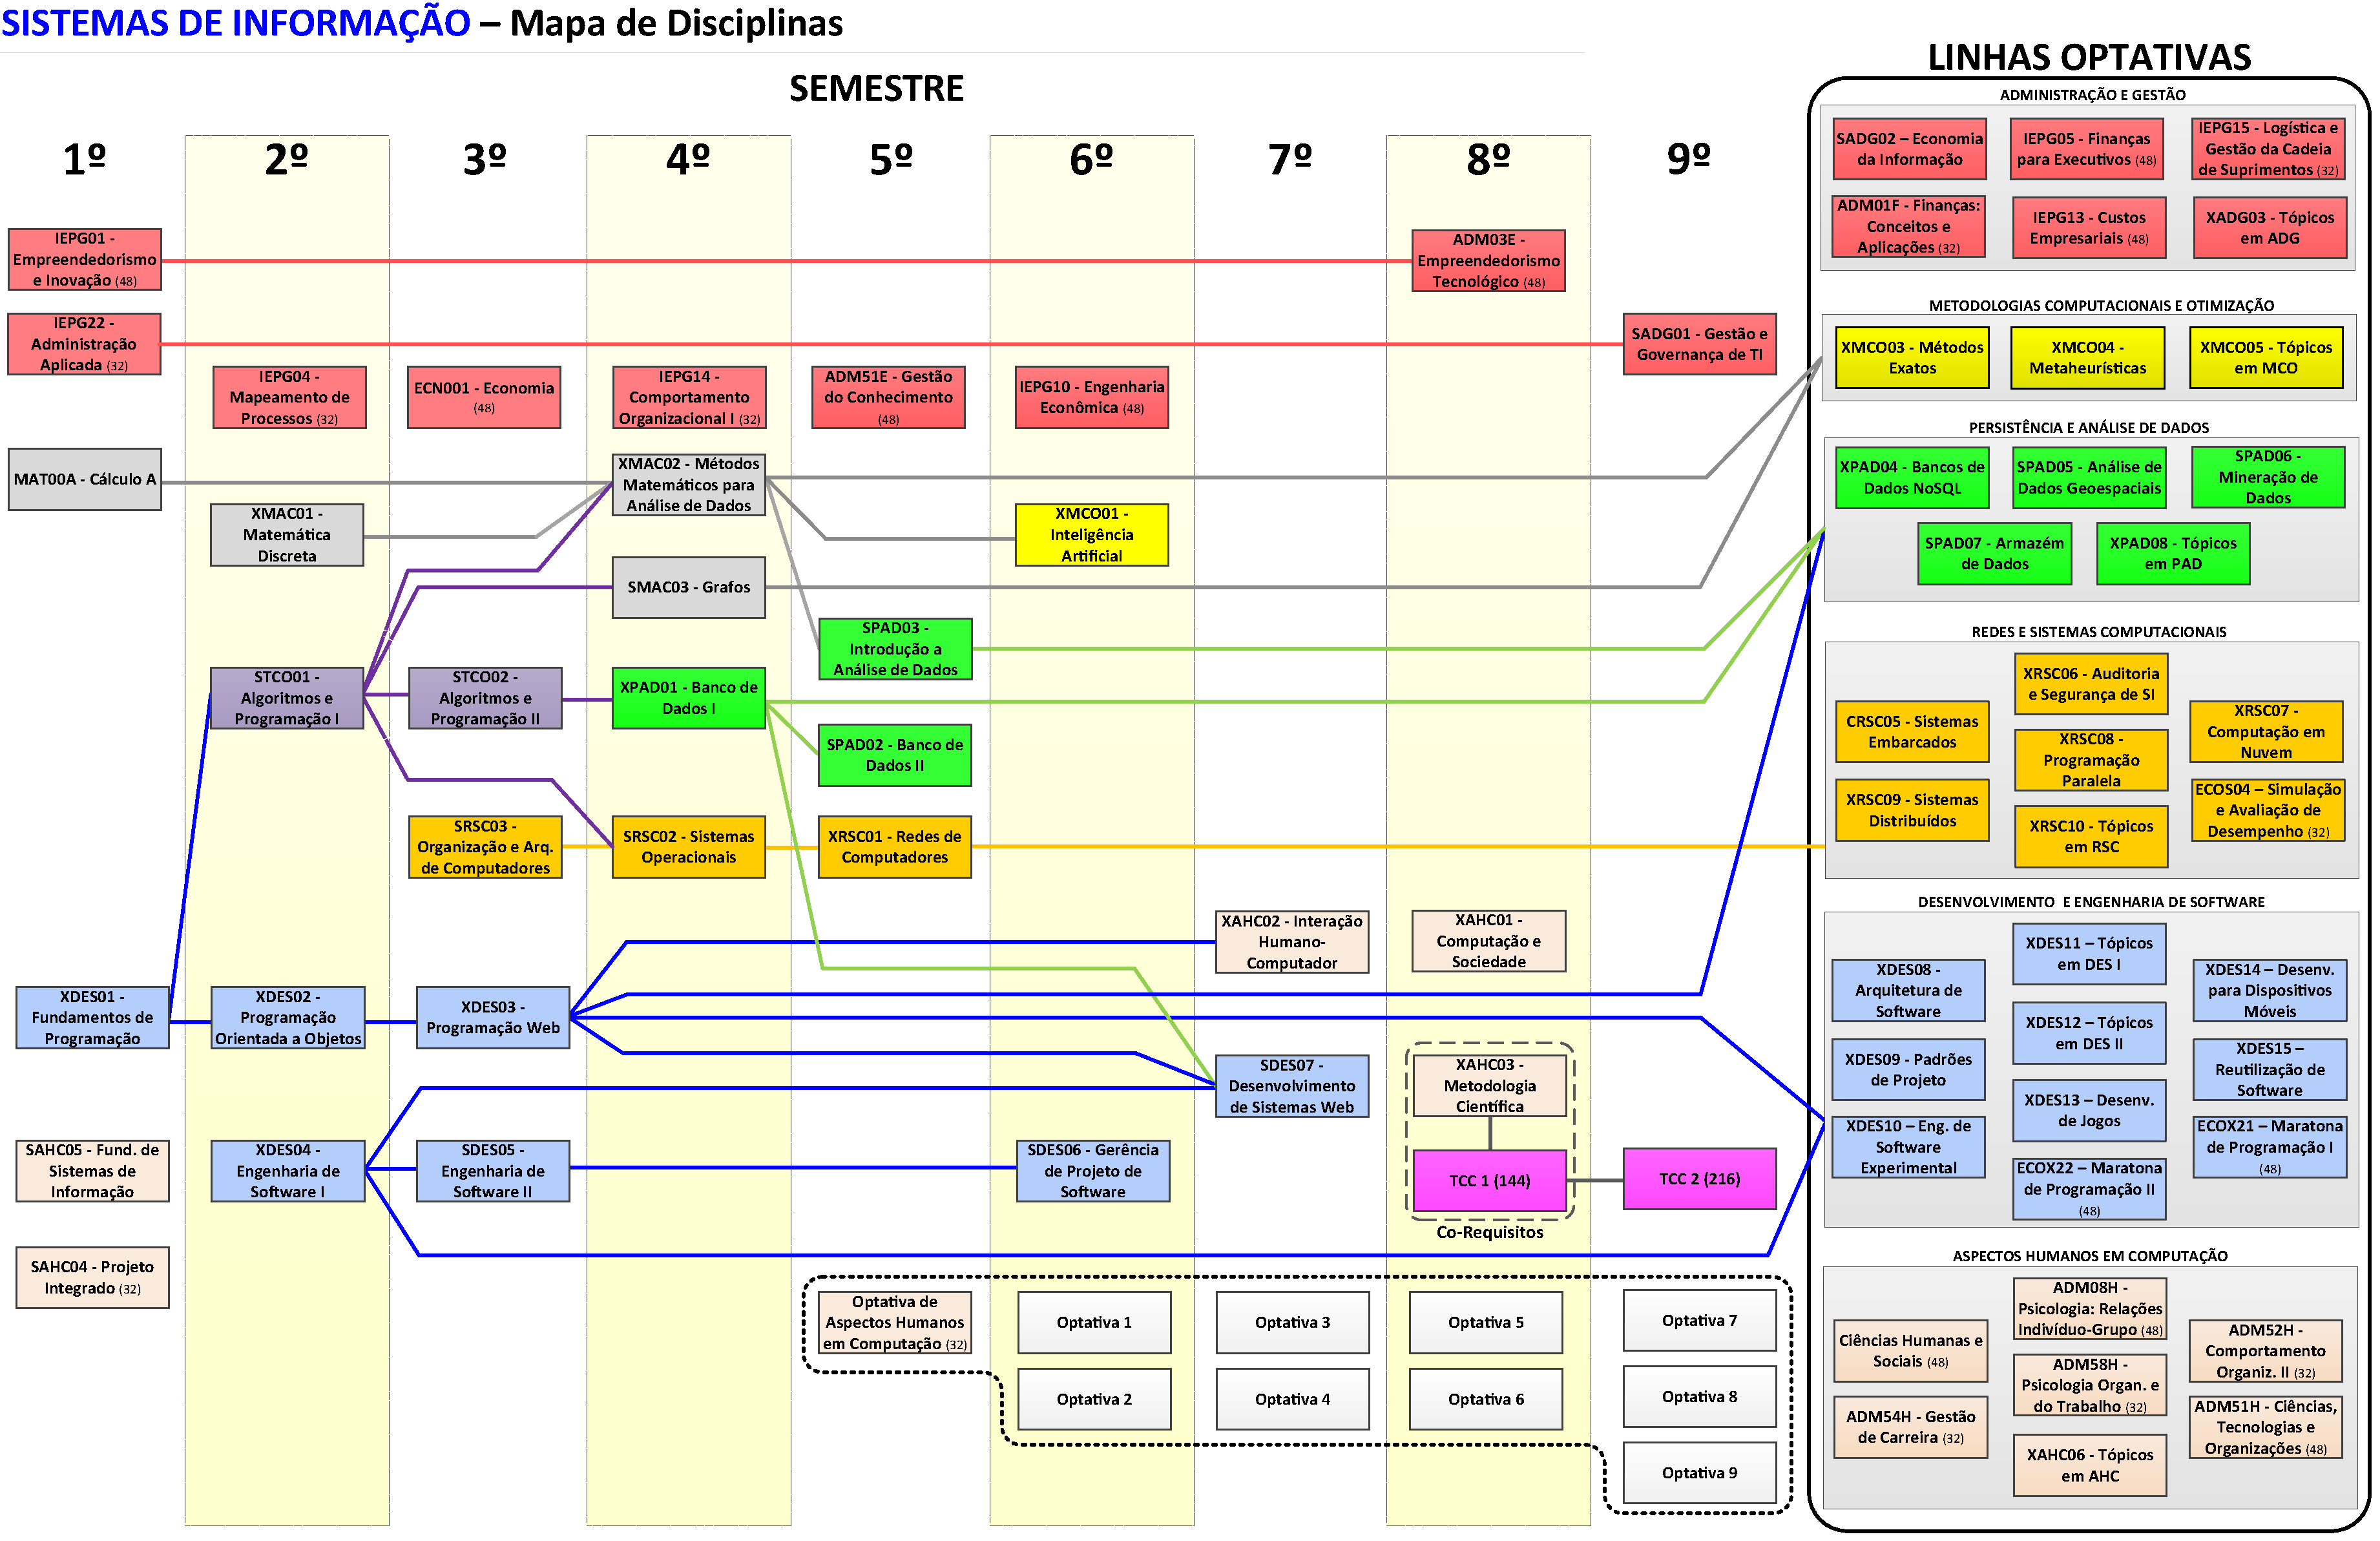
\includegraphics[width=1.0\textwidth]{figs/SIN-MapaDisciplinas.pdf}
    \caption{Exemplo de utilização de uma página configurada como paisagem para figuras ou tabelas muito grandes.}
    \label{fig-Exemplo2}
}

\subsection{Fórmulas Matemáticas}

Consulte o link \url{https://en.wikibooks.org/wiki/LaTeX/Mathematics} que contém diversos conteúdos sobre a construção de fórmulas em \LaTeX, além de símbolos matemáticos. A Equação \ref{eq-Exemplo1} contém um exemplo:

\begin{equation}
	\label{eq-Exemplo1}
	\displaystyle	r_{k+1}(P_{i}) = \sum\limits_{P_{j} \in B_{P_{i}}} \frac{r_{k}(P_{j})}{|P_{j}|}
\end{equation}

A Equação \ref{eq-Exemplo2} é um outro exemplo (OBS. Todas as variáveis de uma fórmula precisam ser descritas no texto):

\begin{equation}
f(n) =
  \begin{cases}
    n/2       & \quad \text{se } n \text{ é ímpar}\\
    -(n+1)/2  & \quad \text{se } n \text{ é par}
  \end{cases}
  \label{eq-Exemplo2}
\end{equation}

\subsection{Códigos-fonte}

Embora um algoritmo, como mostrado na Seção~\ref{ssec:alg}, seja uma das maneiras mais elegantes de se apresentar uma implementação de software, existem algumas situações em que pode ser necessário incluir um código-fonte (ou parte dele) no texto. 

Esta ação pode ser realizada através do comando \noindent\textcolor{blue}{\texttt{$\backslash$lstinputlisting}}. De modo análogo às figuras e tabelas, todos os códigos também são numerados e devem estar citados no texto. Por exemplo: o programa ilustrado pelo Código~\ref{bubblePy} foi inserido no documento através do seguinte comando:

\noindent\textcolor{blue}{\texttt{$\backslash$lstinputlisting[language=Python, caption=\{Implementação do algoritmo Bubble Sort\}, label=bubblePy]\{./elemtextuais/bubble.py\}}}

\lstinputlisting[language=Python, caption={Implementação do algoritmo Bubble Sort}, label=bubblePy]{./elemtextuais/bubble.py}

Para mais detalhes sobre a inclusão de códigos-fonte, consulte: \url{https://en.wikibooks.org/wiki/LaTeX/Source_Code_Listings}.



